% !TeX root = ../main.tex

\chapter{CE$\nu$NS探测信号模型}

本章将分析反应堆中微子的来源和能谱,以探测器响应为基础建立实验中的信号模型。

\section{反应堆中微子的CE$\nu$NS}

典型的热中子堆(thermal-neutron reactor)中99.7\%以上的反应堆中微子来自于四种主要裂变核素子核(裂变碎片)的衰变:
${}^{235}\mathrm{U},{}^{238}\mathrm{U},{}^{239}\mathrm{Pu},{}^{241}\mathrm{Pu}$\cite{juno_collaboration_tao_2020}。
反应堆中可裂变核素均为富中子核素,其裂变碎片也是富中子核素,可以发生$\beta$衰变放出电子($\beta$射线)和电子反中微子。
每一次核裂变后会伴随约6次$\beta$衰变和中微子发射,热中子堆每吉瓦($10^{9}\si{W},\si{GW}$)热功率将每秒产生$2\times10^{20}$个电子反中微子。
这些中微子的能谱是几千种裂变碎片的$\beta$衰变中微子能谱的叠加,见图\ref{fig:fission}。裂变产物的复杂性对于精确地计算反应堆中微子能谱是不利的。

\begin{figure}
  \begin{subfigure}{.3\textwidth}
    \centering
    \includesvg[width=1.0\linewidth]{figures/Nuclear_fission.svg}
    \caption{\label{fig:nuclear_fission} 典型的${}^{235}\mathrm{U}$裂变过程}
  \end{subfigure}
  \begin{subfigure}{.7\textwidth}
    \centering
    \includesvg[width=1.0\linewidth]{figures/fission_yield.svg}
    \caption{\label{fig:fission_yield} ${}^{235}\mathrm{U}$和${}^{239}\mathrm{Pu}$的热中子裂变产额}
  \end{subfigure}
  \caption{\label{fig:fission} 热中子堆中的裂变过程。典型裂变核素${}^{235}\mathrm{U}$的产物,如${}^{92}\mathrm{Kr}$和${}^{141}\mathrm{Ba}$均为$\beta$衰变核素,见图\subref{fig:nuclear_fission};裂变碎片成分十分复杂,热中子裂变条件下,${}^{235}\mathrm{U}$和${}^{239}\mathrm{Pu}$裂变碎片的质量与产额关系中,碎片质量将以裂变核素质量的一半为轴,几乎左右对称,并形成两个峰\cite{crouch_fission-product_1977},见图\subref{fig:fission_yield}。}
\end{figure}

目前有两种反应堆中微子能谱模型。2011年前,最常用的反应堆中微子能谱为ILL-Vogel模型,其中${}^{235}\mathrm{U}$、${}^{239}\mathrm{Pu}$和${}^{241}\mathrm{Pu}$的
能谱反推自1980年代在ILL(the Institut Laue-Langevin)的裂变产物$\beta$能谱测量\cite{von_feilitzsch_experimental_1982,schreckenbach_determination_1985,hahn_antineutrino_1989},
因${}^{238}\mathrm{U}$裂变主要由快中子引发,难以直接测量,其中微子能谱来自P.Vogel的理论计算\cite{p_vogel_neutrino_1989}。
ILL-Vogel模型与2011年前的反应堆中微子实验的结果吻合\cite{an_improved_2017}。
2011年后P.Huber和T.A.Mueller等人引入了更精细的理论计算\cite{huber_determination_2011,mueller_improved_2011},称为Huber-Mueller模型,
得到的中微子能谱相对于测量结果有超出。

在灵敏度预测中高能(超过2$\si{MeV}$)中微子的能谱$s_i(E_\nu)$输入($i=1\cdots4$,遍历四种裂变核素),将使用Huber-Mueller模型,其中${}^{235}\mathrm{U}$、${}^{239}\mathrm{Pu}$和${}^{241}\mathrm{Pu}$参考P.Huber的计算结果\cite{huber_determination_2011},${}^{238}\mathrm{U}$参考T.A.Mueller的计算结果\cite{mueller_improved_2011};
在低能($0-2\si{MeV}$)区域,将使用P.Vogel的理论计算能谱\cite{p_vogel_neutrino_1989},见图\ref{fig:neutrino_energy_spectrum}。本文中将反应堆将只以裂变产物$\beta$衰变放出的电子反中微子作为中微子源。

\begin{figure}
    \centering
    \includesvg[width=0.7\linewidth]{figures/neutrino_energy_spectrum.svg}
    \caption{\label{fig:neutrino_energy_spectrum} 灵敏度预测中使用的各种核素的中微子能谱,
    因逆$\beta$衰变反应有约$1.8\si{MeV}$的阈值,所以虽然低能中微子占总流强的主要部分,但未被Daya Bay等反应堆中微子实验测量到\cite{an_improved_2017}。}
\end{figure}

为了计算反应堆中微子的总能谱和总流强,需要引入裂变核素每次裂变的平均释放能量$e_i$,已有较精确的理论计算\cite{ma_improved_2013},见表\ref{tab:per_fission}:

\begin{table}
  \centering
  \caption{四种主要裂变核素每次裂变释放的平均能量和裂变份额}
  \begin{tabular}{ccc}
    \toprule
    核素 & $e_i(\si{MeV})$ & $f_i$ \\
    \midrule
    ${}^{235}\mathrm{U}$ & 202.36 & 0.561 \\
    ${}^{238}\mathrm{U}$ & 205.99 & 0.076 \\
    ${}^{239}\mathrm{Pu}$ & 211.12 & 0.307 \\
    ${}^{241}\mathrm{Pu}$ & 214.26 & 0.056 \\
    \bottomrule
  \end{tabular}
  \label{tab:per_fission}
\end{table}

有了以上基础,反应堆中微子的能谱定义为:

\begin{align}
    \label{eq:sum_spectrum}
    \phi\left(E_\nu,t\right) &= \frac{W(t)}{\sum_i f_i(t)e_i}\sum_i f_i(t)s_i(E_\nu)
\end{align}

其中$t$为反应堆运行时间,$W(t)$为反应堆运行功率,其与堆芯实际运行状态有关\cite{juno_collaboration_tao_2020};
$f_i(t)$为裂变份额(fission fraction),指四种核素的裂变次数在总裂变次数中的占比,见表\ref{tab:per_fission}。
典型的商用热中子堆中,${}^{235}\mathrm{U}$和${}^{239}\mathrm{Pu}$的裂变份额占主要部分。

裂变份额与核燃料的燃耗(burn-up),即消耗掉的燃料数量,以及燃耗深度(burn-up depth)有关。对于以富集铀作为核燃料的热中子堆,随着${}^{235}\mathrm{U}$的裂变消耗,
可转换材料如${}^{238}\mathrm{U}$会俘获中子转换为易裂变同位素${}^{239}\mathrm{Pu}$,
使得堆内$\mathrm{U}$元素逐渐消耗,$\mathrm{Pu}$元素逐渐累积,见图\ref{fig:fission_fraction}。

\begin{figure}
    \centering
    \includesvg[width=0.7\linewidth]{figures/fission_fraction.svg}
    \caption{\label{fig:fission_fraction} 大亚湾核电站反应堆一个典型的核燃料循环中,裂变份额随着燃耗深度的变化\cite{an_evolution_2017}。}
\end{figure}

在本文中,简化考虑反应堆能谱形状和绝对强度的时间演化,即认为$f_i(t)=f_i,W(t)=W$。
LXeTPC实验将选址在山东石岛湾核电站(Shidao Bay Nuclear Power Plant)的某机组附近,预计届时将以$W=0.25\si{GW}$堆芯作为中微子源,在堆芯距离约$12\si{m}$位置放置探测器。实验选址如图\ref{fig:shidaowan}。

\begin{figure}
    \centering
    % 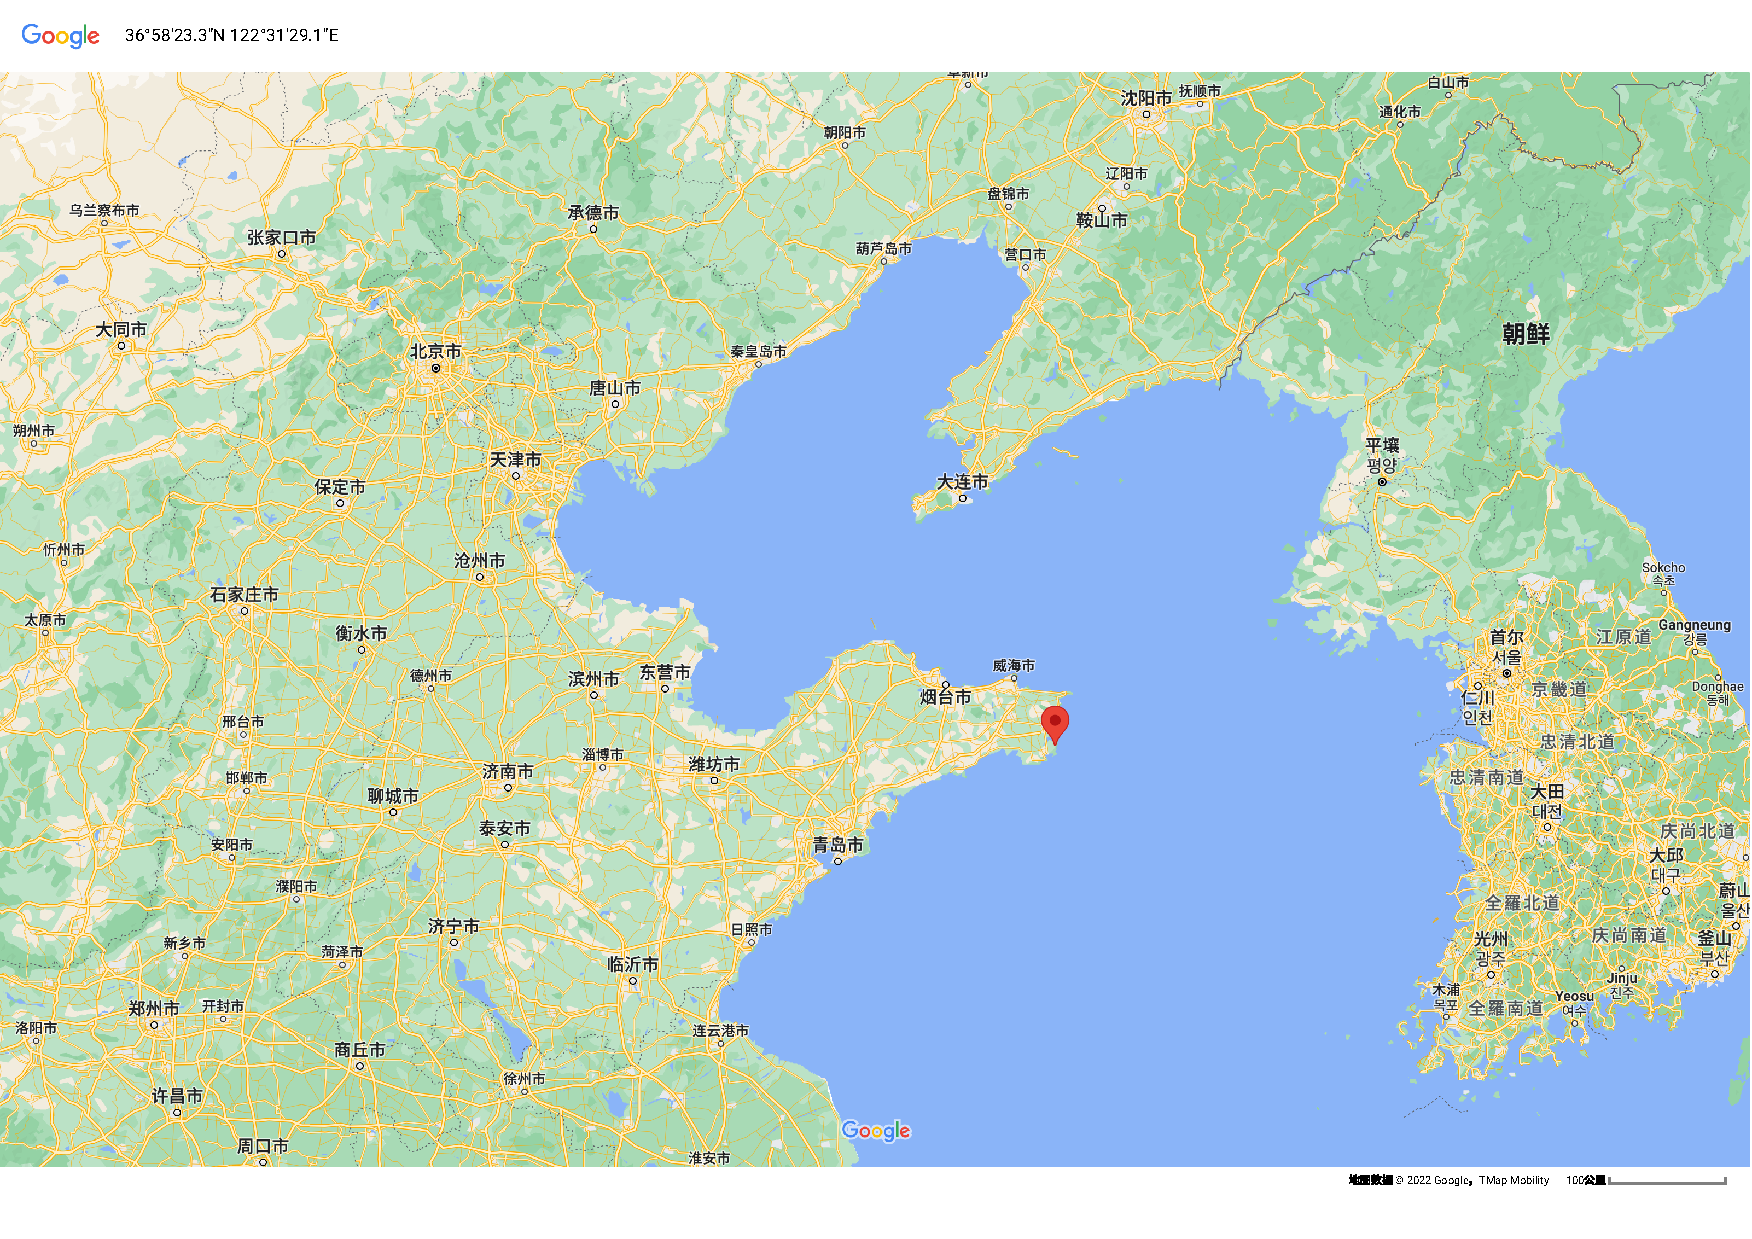
\includepdf[width=0.7\linewidth]{figures/shidaowan.pdf}
    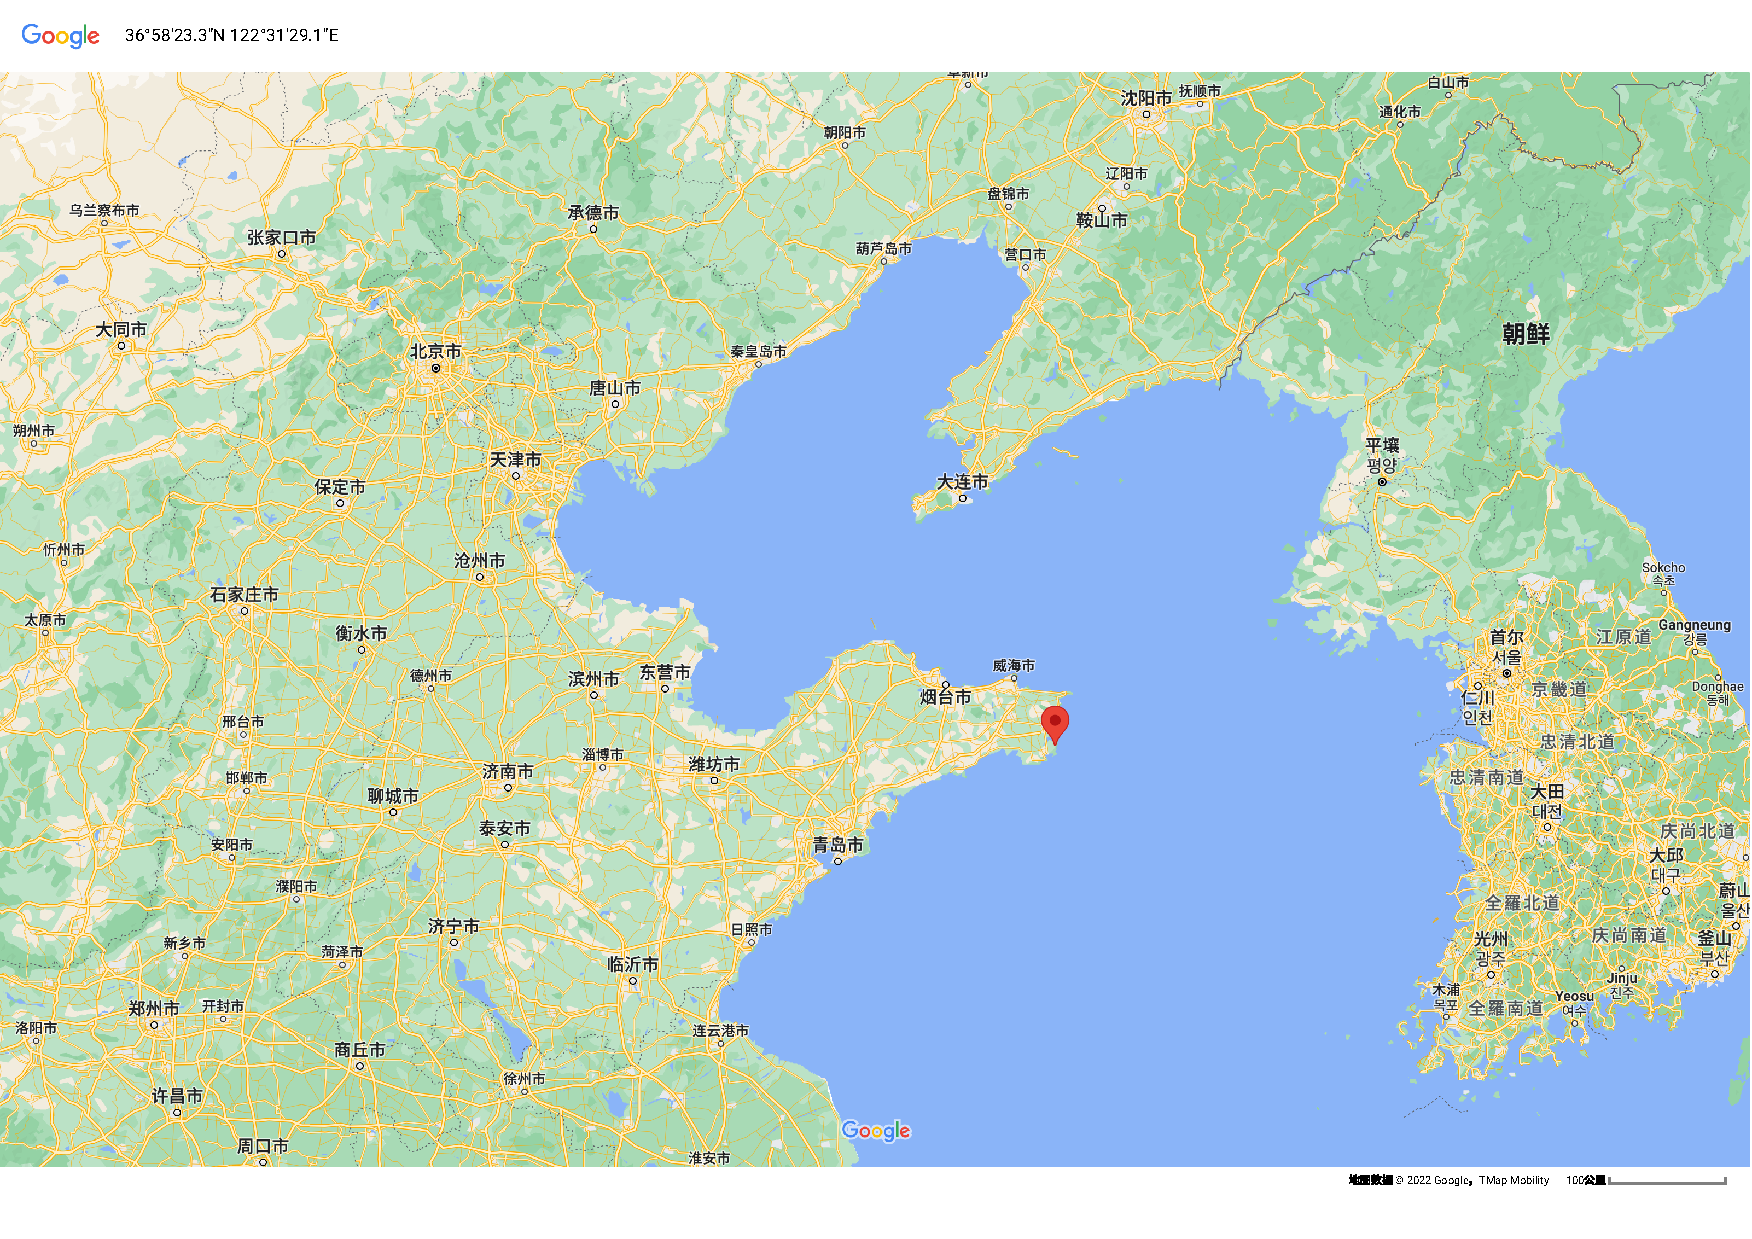
\includegraphics[width=1.0\linewidth]{figures/shidaowan.pdf}
    \caption{\label{fig:shidaowan} 计划中的LXeTPC实验的选址位置。图片来源:Google Maps.\cite{shidaowan_googlemap_220524}。}
\end{figure}

至此我们可以计算得到总的反应堆中微子能谱$\phi\left(E_\nu\right)$,如图\ref{fig:neutrino_flux_spectrum}:

\begin{figure}
    \centering
    \includesvg[width=0.7\linewidth]{figures/neutrino_flux_spectrum.svg}
    \caption{\label{fig:neutrino_flux_spectrum} 石岛湾核电站反应堆中微子能谱,只考虑单堆芯。
    在堆芯距离12$\si{m}$处,反应堆中微子总通量可以达到$2.5\times 10^{12}\si{cm^{-2}s^{-1}}$,
    作为对比,JUNO-TAO实验选址的台山核电站(热功率$4.6\si{GW}$)堆芯附近$30\si{m}$处中微子总通量可以达到$7.4\times 10^{12}\si{cm^{-2}s^{-1}}$\cite{juno_collaboration_tao_2020}。}
\end{figure}

反应堆中微子通过探测器时,探测介质与中微子发生CE$\nu$NS反应的事例率与中微子能量的关系为$S'(E_\nu)$:

\begin{align}
    \label{eq:sevent_rate}
    S'(E_\nu) &= \frac{\phi(E_\nu)}{4\pi L^2}\sum_j N_j\cdot \sigma_j(E_\nu)
\end{align}

其中$N_j$为每单位质量探测介质中原子核数目,单位为$\si{kg^{-1}}$,$j$遍历介质中的不同同位素,对于氙,有${}^{129}\mathrm{Xe},{}^{131}\mathrm{Xe},{}^{132}\mathrm{Xe}$等几种,
对于锗${}^{70}\mathrm{Ge},{}^{72}\mathrm{Ge},{}^{74}\mathrm{Ge}$等几种,同位素丰度可以简单地从公开数据集中获取;
$E_\nu$为中微子能量,$\phi(E_\nu)$为中微子能谱。计算中不考虑反应堆中微子随燃耗深度的演化。

但是在探测中,我们不仅考察总事例率,也会考察可观测物理量,如核反冲能$T_{\mathrm{nr}}$、光子和电子数目($\mathrm{S1}$和$\mathrm{S2}$)的分布,
其中事例率$S(T_{\mathrm{nr}})$与$T_{\mathrm{nr}}$的关系为:
\begin{align}
    \label{eq:tnr_event_rate}
    S(T_{\mathrm{nr}}) &= \frac{1}{4\pi L^2}\int\phi(E_\nu)\sum_j N_j\cdot \frac{\mathrm{d}\sigma_j(E_\nu)}{\mathrm{d}T}\mathrm{d}E_\nu
\end{align}

\begin{figure}
    \centering
    \includesvg[width=1.0\linewidth]{figures/cevns_event_rate.svg}
    \caption{\label{fig:cevns_event_rate} 氙(左图)与锗(右图)两种介质探测CE$\nu$NS的核反冲能分布(事例率)。
    因为氙原子核普遍比锗原子核重,所以以氙为介质的核反冲能谱向低能偏移。
    不考虑探测效率,氙探测器中$0.5\si{keV_{\mathrm{nr}}}$以上的核反冲可以达到$228.1\si{kg^{-1}y^{-1}}$,
    锗探测器中$1.0\si{keV_{\mathrm{nr}}}$以上的核反冲可以达到$69.3\si{kg^{-1}y^{-1}}$。}
\end{figure}

\section{LXeTPC探测CE$\nu$NS信号}
\label{sec:lxe_signal}

第\ref{sec:basic_response}章中讨论过液氙中基本的微观过程,在本文简化的信号模型中,$\mathrm{S1}$和$\mathrm{S2}$由一系列正比过程决定,
如图\ref{fig:signal_flow}。

\begin{figure}
    \centering
    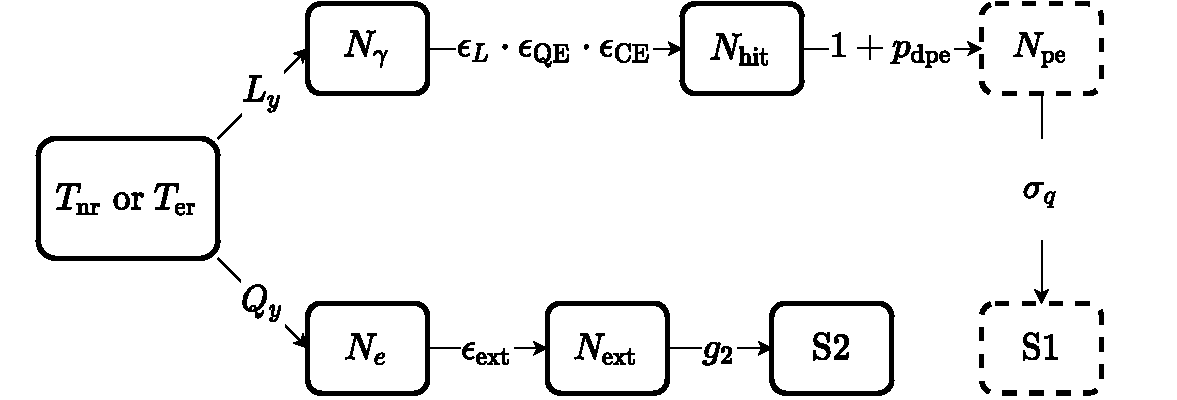
\includegraphics[width=1.0\linewidth]{figures/signal_flow.pdf}
    \caption{\label{fig:signal_flow} LXeTPC 中的信号传递过程。
    首先沉积的核反冲能量$T_{\mathrm{nr}}$或电子反冲能量$T_{\mathrm{er}}$转化为量子数:光子数$N_\gamma$和电子数$N_e$,
    光子在传递过程中的衰减由乘积$\epsilon_L\cdot\epsilon_\mathrm{QE}\cdot\epsilon_\mathrm{CE}$描述,并转化为PMT击中数$N_\mathrm{hit}$;
    电子在门电极和阳极之间被拉出可能有一定损失,最终倍增$g_2$倍称为被探测到的光电子数目$S2$。}
\end{figure}

光子数$N_\gamma$和电子数$N_e$用光电产额描述:

\begin{align}
    \label{eq:N_ge_lq}
    N_\gamma &\sim \mathrm{Poisson}\left(\varepsilon\cdot L_y\right) \\
    N_e &\sim \mathrm{Poisson}\left(\varepsilon\cdot Q_y\right)
\end{align}

其中成绩能量$\varepsilon$可以取$T_{\mathrm{nr}}$或$T_{\mathrm{er}}$。
电子反冲的光电产额用NEST模型描述:

\begin{figure}
    \centering
    \includesvg[width=1.0\linewidth]{figures/lxe_er_yield.svg}
    \caption{\label{fig:lxe_er_yield} NEST模型中的低能电子反冲光电产额\cite{lenardo_global_2015,jason_brodsky_chris_tunnell_mszydagis_jbalajth_vetri_velan_junying_huang_2019}。}
\end{figure}

2020年XENON1T实验测量了太阳${}^{8}B$中微子的CE$\nu$NS信号\cite{aprile_search_2021},本文中液氙中低能核反冲光电产额使用该结果:

\begin{figure}
    \centering
    \includesvg[width=1.0\linewidth]{figures/lxe_nr_yield.svg}
    \caption{\label{fig:lxe_nr_yield} 低能核反冲光电产额\cite{aprile_search_2021,jason_brodsky_chris_tunnell_mszydagis_jbalajth_vetri_velan_junying_huang_2019},
    本文信号模型中采用2020年XENON1T的结果,NEST模型提供的核反冲产额与其有一定差异。}
\end{figure}

\subsection{S2-Only分析}

S2-Only 分析为仅使用$\mathrm{S2}$作为似然函数(likelihood function)分析维度的物理分析。
一般在$\mathrm{S1}$信息较少或不存在的情况下使用。对于反应堆中微子,其产生的核反冲能量较低,
CE$\nu$NS事件大多不具有$\mathrm{S1}$或者$\mathrm{S1}$探测效率很低,所以主要采用S2-Only 分析。

电子漂移到气液交界面处后,被提出液面的过程中可能有少量损耗,
用概率为$\epsilon_\mathrm{ext}$的二项分布描述,见\ref{eq:N_ext},本文中取$\epsilon_\mathrm{ext}=1$。
强电场对提出电子的倍增过程用参数为$(g_2,\Delta g_2)$的正态分布描述:

\begin{align}
    \label{eq:s2}
    \mathrm{S2} &\sim \mathrm{Gauss}\left(g_2,\sqrt{N_\mathrm{ext}}\cdot\Delta g_2\right)
\end{align}

其中取$g_2=20,\Delta g_2=6.67$。由此我们可以计算得到CE$\nu$NS事件的电子谱和$\mathrm{S2}$分布,
比较信号本底在分析维度上的分布,对确定感兴趣的分析区域(region of interest, ROI)很重要,如图\ref{fig:S2eS2_rate}:

\begin{figure}
  \begin{subfigure}{.5\textwidth}
    \centering
    \includesvg[width=1.0\linewidth]{figures/S2e_rate.svg}
    \caption{\label{fig:S2e_rate} CE$\nu$NS事件中的电子个数$N_e$谱}
  \end{subfigure}
  \begin{subfigure}{.5\textwidth}
    \centering
    \includesvg[width=1.0\linewidth]{figures/S2_rate.svg}
    \caption{\label{fig:S2_rate} CE$\nu$NS事件中的$\mathrm{S2}$分布}
  \end{subfigure}
  \caption{\label{fig:S2eS2_rate} CE$\nu$NS事件中的电子个数$N_e$和$\mathrm{S2}$分布。
  随着$N_e$或$\mathrm{S2}$上升,分布的权重迅速降低,说明对低能事件的探测对实验至关重要。
  两图中浅蓝色阴影是感兴趣的分析区域,其上阈将在第\ref{sec:backgrounds}章中讨论。}
\end{figure}

降低探测器的能量下阈对十分重要。本文灵敏度计算中认为探测器对4个及以上的电子的探测效率为100\%;
对更小的$\mathrm{S2}$,一方面探测效率低,另一方面,更低能区可能存在无法成功建模的本底,所以不予考虑;
对应的$\mathrm{S2}$下阈取$80\mathrm{PE}$。

低能反应堆中微子在探测器沉积的能量有更小的几率产生超过$\mathrm{S2}$下阈信号,
所以通过CE$\nu$NS反应道测量的反应堆中微子大多具有较高能量,见图\ref{fig:neutrino_efficiency}。

\begin{figure}
    \centering
    \includesvg[width=0.7\linewidth]{figures/neutrino_efficiency.svg}
    \caption{\label{fig:neutrino_efficiency} $\mathrm{S2}$下阈取$80\mathrm{PE}$时探测到的CE$\nu$NS信号对应的中微子能量分布。
    可见没有$4\si{MeV}$以下的中微子被探测到,CE$\nu$NS测量将有可能对反应堆中微子高能区域能谱的理论计算敏感。}
\end{figure}

\subsection{S1-S2分析}

尽管CE$\nu$NS信号的$\mathrm{S1}$保留信息较少,但仍然可以通过单独分析包含$\mathrm{S1}$的信号,
来限制某些与光信号有关的物理过程,如低能核反冲的光产额。

光子在液氙中的光传输过程和损耗由乘积$\epsilon_\mathrm{hit}=\epsilon_L\cdot\epsilon_\mathrm{QE}\cdot\epsilon_\mathrm{CE}$描述:

\begin{align}
    \label{eq:N_hit}
    N_\mathrm{hit} &\sim \mathrm{Binom}\left(N_\gamma,\epsilon_L\cdot\epsilon_\mathrm{QE}\cdot\epsilon_\mathrm{CE}\right)
\end{align}

本文中$\epsilon_\mathrm{hit}$取较保守的$0.08\si{hit\cdot ph^{-1}}$。

\begin{align}
    \label{eq:N_peS1}
    N_\mathrm{pe} - N_\mathrm{hit} &\sim \mathrm{Binom}\left(N_\mathrm{hit},p_\mathrm{dpe}\right) \\
    \mathrm{S1} &\sim \mathrm{Gauss}\left(N_\mathrm{pe},\sqrt{N_\mathrm{pe}}\cdot\sigma_q\right)
\end{align}

双光电子概率$p_\mathrm{dpe}$取为0.2,PMT电荷分布的展宽用正态分布或伽马分布(Gamma distribution)描述,其标准差$\sigma_q$取为0.5。
但实际上反应堆中微子能产生的$T_\mathrm{nr}$很低,产生的光信号很少,$\mathrm{S1}$携带信息较少,后续所有分析仅在$N_\mathrm{hit}$维度进行。

对于较小的$\mathrm{S1}$,触发和波形分类效率较低,我们使用接收率曲线来描述探测效率,如图\ref{fig:s1_hits_pe}。

\begin{figure}
    \centering
    \includesvg[width=1.0\linewidth]{figures/s1_hits_pe.svg}
    \caption{\label{fig:s1_hits_pe} CE$\nu$NS信号$N_\mathrm{hit}$和$\mathrm{S1}$的接收率(左图),
    CE$\nu$NS信号$N_\mathrm{hit}$分布(右图,同时要求$\mathrm{S2}>80\si{PE}$)。接收率曲线在$N_\mathrm{hit}\le1$时取0。
    $N_\mathrm{hit}$主要集中在$N_\mathrm{hit}=2$的bar中。}
\end{figure}

因$N_\mathrm{hit}$分布较窄,后续S1-S2分析中仍将以$\mathrm{S2}$为分析维度,只要求S1-S2事件的$N_\mathrm{hit}\ge2$。
具体分析流程将在第\ref{sec:sensitivity}章中详细讨论。

表\ref{tab:lxe_tpc_parameters}为LXeTPC探测CE$\nu$NS信号过程中设置的探测器参数取值:

\begin{table}
  \centering
  \caption{探测CE$\nu$NS的LXeTPC参数取值}
  \begin{tabular}{ccc}
    \toprule
    符号 & 物理量 & 取值 \\
    \midrule
    $L_y$ & 光子产额 & 图\ref{fig:lxe_nr_yield} \\
    $Q_y$ & 电子产额 & 图\ref{fig:lxe_nr_yield} \\
    $\epsilon_\mathrm{hit}$ & PMT击中效率 & 0.08 \\
    $p_\mathrm{dpe}$ & PMT双光电子概率 & 0.2 \\
    $\epsilon_\mathrm{ext}$ & 电子提取效率 & 1.0 \\
    $g_2$ & $\mathrm{S2}$电子等效的平均光电子数 & $20\si{PE/\mathrm{e}^-}$ \\
    $\Delta g_2$ & $\mathrm{S2}$电子等效的光电子数的标准差 & $6.67\si{PE/\mathrm{e}^-}$ \\
    \bottomrule
  \end{tabular}
  \label{tab:lxe_tpc_parameters}
\end{table}

\section{HPGe探测器的CE$\nu$NS信号}
